% !TeX root = ../main.tex
\chapter{架构}\label{ch5}

多年来,深度学习领域已经为每个应用领域开发了多种深度架构,这些架构在多个人们关注的标准方面表现出良好的折中:例如 训练便捷性、预测准确性、内存占用、计算成本、可扩展性等。

\section{多层感知机}\label{sec5.1}

最简单的深度架构是\keyterm{多层感知机}(\keyterm{MLP}),它由一系列\keyterm{全连接层}组成,层与层之间通过\keyterm{激活函数}分隔。请参见图 \ref{fig5.1} 中的示例。由于历史原因,在这样的模型中,\keyterm{隐藏层}的数量指的是线性层的数量,不包括最后一层。

\begin{figure}
    \centering
    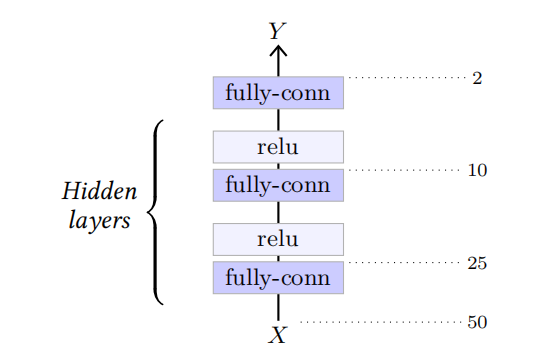
\includegraphics[width=0.9\textwidth]{fig/fig5.1.png}
    \caption[多层感知机]{该多层感知器以大小为 $50$ 的一维张量作为输入,由三个全连接层组成,输出维度分别为 $25$、$10$ 和 $2$,前两个层后面是 ReLU 层。}
    \label{fig5.1}
\end{figure}

一个关键的理论成果是\keyterm{通用逼近定理} \citep{Cybenko1989},该定理指出,如果激活函数 $\sigma$ 是连续的且非多项式的,那么任意连续函数 $f$ 都可以在紧致域上被形式为 $l_2 \circ \sigma \circ l_1$ 的模型任意精确地一致逼近,其中紧致域是有界的并包含其边界,$l_1$ 和 $l_2$ 是仿射的。这样的模型是一个只有单个隐藏层的多层感知机(\keyterm{MLP}),这个结果意味着它可以近似任何具有实用价值的东西。然而,这种逼近成立的条件是第一个线性层的输出维度可以任意大。

尽管 MLP 很简单,但当要处理的信号维度不太大时,它仍然是一个重要的工具。

\section{卷积网络}\label{sec5.2}

处理图像的标准架构是\keyterm{卷积网络},也称 \keyterm{convnet},它结合了多个\keyterm{卷积层},既可以在信号被\keyterm{全连接层}处理之前降低信号大小,也可以输出一个同样较大尺寸的二维信号。

\subsubsection*{类 LeNet}

用于图像\keyterm{分类}的原始 \keyterm{LeNet} \citep{Lecun98} 模型结合了一系列充当特征提取器角色的二维\keyterm{卷积层}和\keyterm{最大池化}层,以及一系列充当 \keyterm{MLP} 并实际执行分类任务的\keyterm{全连接层}(见图 \ref{fig5.2})。

\begin{figure}
    \centering
    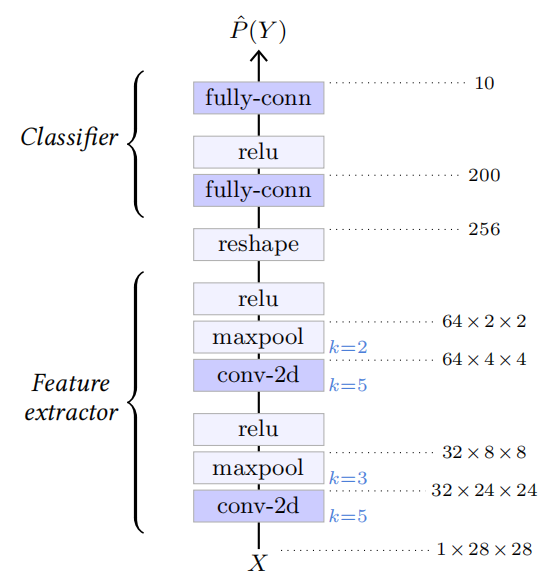
\includegraphics[width=0.9\textwidth]{fig/fig5.2.png}
    \caption[类 LeNet 卷积模型]{用于对手写数字的 $28 \times 28$ 灰度图像进行分类的小型 \keyterm{LeNet} 网络示例 \citep{Lecun98}。它的前半部分是卷积层,交替使用卷积层和最大池化层,将信号维度从 $28 \times 28$ 个标量减少到 $256$。它的后半部分通过一个隐藏层感知器处理这个 $256$ 维特征向量,以计算 $10$ 个 logit 分数对应十个可能的数字。}
    \label{fig5.2}
\end{figure}

这一架构为许多具有相同结构的模型提供了蓝图,这些模型只是在规模上更大大,例如 AlexNet \citep{nips-1502.c399862d3b9d6b76c8436e924a68c45b} 或 VGG系列 \citep{arxiv-1409.1556}。

\subsubsection*{残差网络}

遵循 LeNet 家族架构的标准卷积神经网络不易于扩展为深层架构,并且会遇到梯度消失问题。\citep{arxiv-1512.03385} 提出的 \keyterm{残差网络}(ResNets)明确解决了梯度消失问题,它们通过\keyterm{残差连接}(详见 \ref{sec4.7} 节),使得网络能够拥有数百层。残差网络已成为计算机视觉应用的标准架构,并且根据层数的不同存在多个版本。我们将详细探讨用于分类的 \keyterm{ResNet-50} 架构。

\begin{figure}
    \centering
    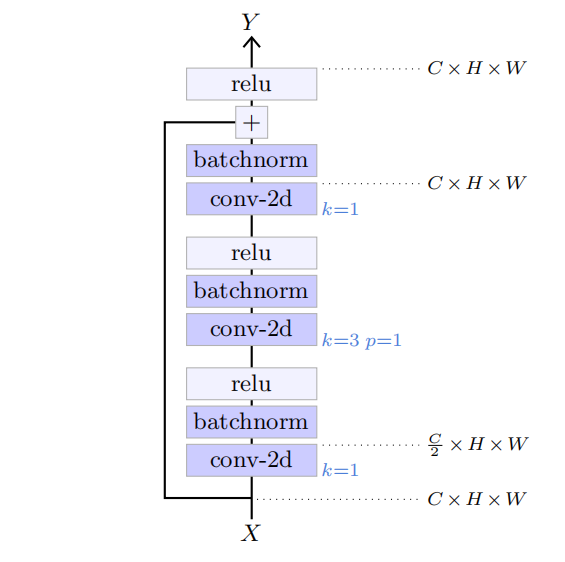
\includegraphics[width=0.9\textwidth]{fig/fig5.3.png}
    \caption[残差块]{残差块}
    \label{fig5.3}
\end{figure}

与其他 ResNet 一样,ResNet-50 由一系列\keyterm{残差块}组成,每个残差块结合了多个\keyterm{卷积层}、\keyterm{批归一化}层和 ReLU 层,并包裹在残差连接中。如图 \ref{fig5.3} 所示。

在处理真实图像时,要实现高性能的一个关键要求是传递具有大量通道的信号,以允许丰富的表征。然而,卷积层的参数数量及其计算成本与通道数呈二次方关系。这种残差块通过首先使用 $1 \times 1$ 卷积减少通道数来缓解这一问题,然后在减少的通道数上用 $3 \times 3$ 卷积进行空间操作,之后再次通过 $1 \times 1$ 卷积放大通道数。

\begin{figure}
    \centering
    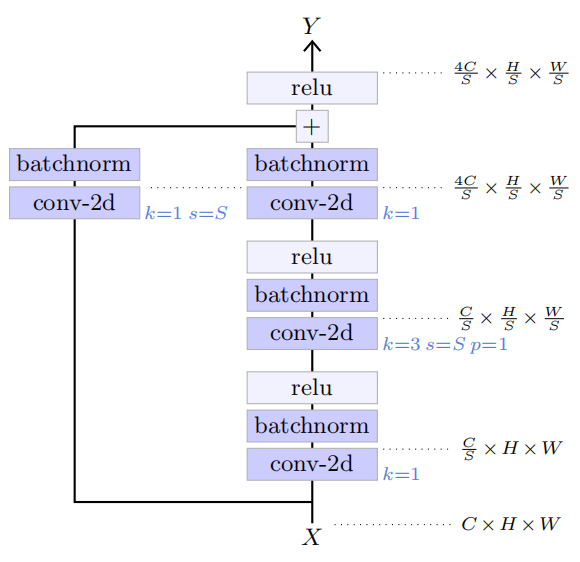
\includegraphics[width=0.9\textwidth]{fig/fig5.4.png}
    \caption[下采样残差块]{下采样残差块接受一个元参数 $S$,即第一个卷积层的步长,用于调节张量尺寸的缩减程度。}
    \label{fig5.4}
\end{figure}

该网络通过减少信号的维度来最终计算用于分类的 logit 值。这得益于一个由几部分组成的架构,每个部分都以一个\keyterm{下采样残差块}开始,其将信号的高度和宽度减半,并将通道数加倍,然后是一系列残差块。这样的下采样残差块具有与标准残差块相似的结构,不同之处在于它需要一个改变张量形状的残差连接。这是通过步长为 $2$ 的 $1 \times 1$ 卷积实现的(参见图 \ref{fig5.4})。

\begin{figure}
    \centering
    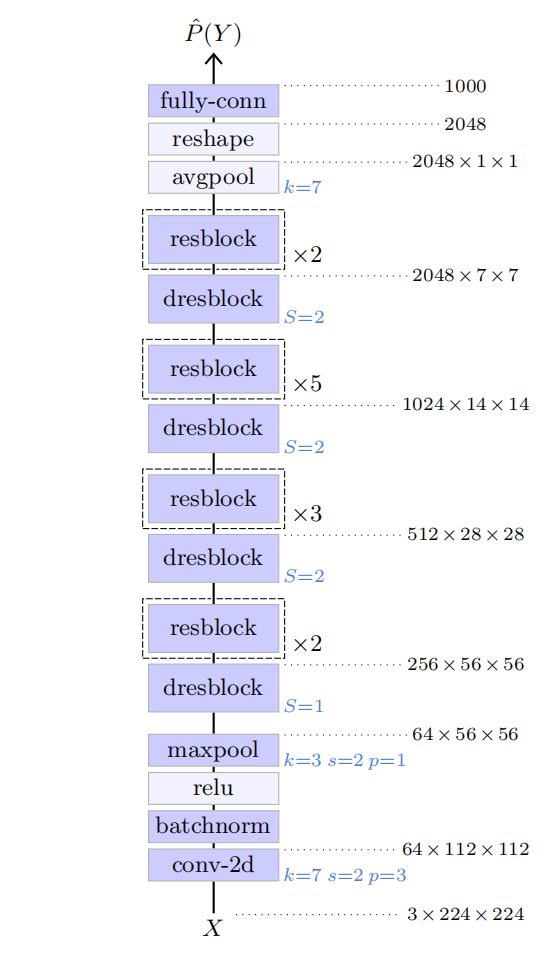
\includegraphics[width=0.9\textwidth]{fig/fig5.5.png}
    \caption[ResNet-50]{ResNet-50 的结构 \citep{arxiv-1512.03385}}
    \label{fig5.5}
\end{figure}

ResNet-50 的整体结构如图 \ref{fig5.5} 所示。 它从 $7 \times 7$ 卷积层开始,将三通道输入图像转换为尺寸减半的 $64$ 通道图像,随后是四部分残差块。令人惊讶的是,在第一部分中,并没有下采样,只是将通道数增加了 $4$ 倍。最后一个残差块的输出是 $2048 \times 7 \times 7$,其通过一个 $7 \times 7$ 核大小的平均池化被转换为 $2048$ 维的向量,然后通过全连接层处理以获得最终的 logit 值,此处为 $1000$ 个类别。

\section{注意力模型}\label{sec5.3}

正如 \ref{sec4.8} 节所述,许多应用,特别是自然语言处理应用,可以从包含注意力机制的模型中受益匪浅。\cite{arxiv-1706.03762} 提出的 \keyterm{Transformer} 是此类任务的首选架构,它对深度学习的最新进展发挥了重要作用。

\subsubsection*{Transformer}

原始的 Transformer,如图 \ref{fig5.7} 所示,设计用于序列到序列的翻译。它结合了一个编码器,用于处理输入序列并获得精炼的表示,以及一个自回归解码器,基于编码器对输入序列的表示以及到目前为止生成的输出 Token 来生成结果序列的每个 Token。

正如 \ref{sec5.2} 节中的残差卷积网络一样,Transformer 的编码器和解码器都是由残差连接构建的复合块序列。

\begin{figure}
    \centering
    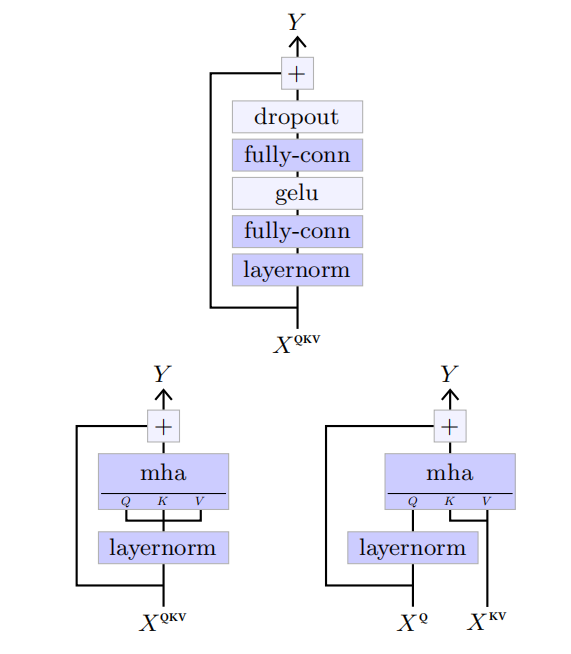
\includegraphics[width=0.9\textwidth]{fig/fig5.6.png}
    \caption[Transformer 组件]{\keyterm{前馈模块}(上)、\keyterm{自注意力模块}(左下)和\keyterm{交叉注意力模块}(右下)。\cite{Radford2018} 提出的这些特定结构与 \cite{arxiv-1706.03762} 的原始架构略有不同,尤其是在残差块中,先进行层归一化处理。}
    \label{fig5.6}
\end{figure}

\begin{itemize}
    \item 图 \ref{fig5.6} 顶部所示的\keyterm{前馈模块}是一个隐藏层 \keyterm{MLP},其前面是一层\keyterm{层归一化}处理。它可以分别更新每个位置的表示。
    \item 图 \ref{fig5.6} 左下角所示的\keyterm{自注意力模块}是一个\keyterm{多头注意力层}(详见 \ref{sec4.8} 节),它能全局重组信息,允许任何位置从任何其他位置收集信息,前面是一层\keyterm{层归一化}处理。如 \ref{sec4.8} 节所述,可以通过在注意力层中使用适当的掩码,来使该模块具有\keyterm{因果性}。
    \item 图 \ref{fig5.6} 右下角所示的\keyterm{交叉注意力模块}与此类似,不同之处在于它接受两个序列作为输入,一个用来计算查询,另一个用来计算键和值。
\end{itemize}

\begin{figure}
    \centering
    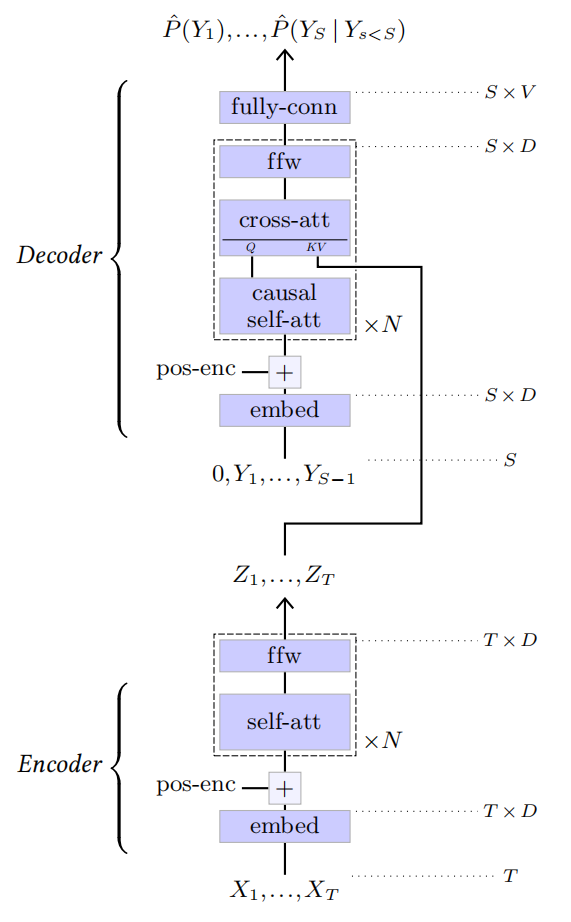
\includegraphics[width=0.9\textwidth]{fig/fig5.7.png}
    \caption[Transformer]{原始的编码器-解码器 \keyterm{Transformer 模型},用于序列到序列的翻译 \citep{arxiv-1706.03762}。}
    \label{fig5.7}
\end{figure}

Transformer 的编码器(参见图 \ref{fig5.7},底部)使用\keyterm{嵌入层}(详见 \ref{sec4.9} 节)重新编码输入的离散 Token 序列 $X_1,\dots,X_T$,并添加\keyterm{位置编码}(详见 \ref{sec4.10} 节),然后通过多个自注意力模块处理,以生成精炼的表示 $Z_1,\dots,Z_T$。

解码器(参见图 \ref{fig5.7},顶部)以到目前为止生成的结果 Token 序列 $Y_1,\dots,Y_{S-1}$ 作为输入,同样通过嵌入层重新编码它们,添加位置编码,并通过交替的\keyterm{因果}自注意力模块和交叉注意力模块进行处理,以产生预测下一个 Token 的 logit 值。这些交叉注意力模块从编码器的结果表示 $Z_1,\dots,Z_T$ 计算它们的键和值,使得生成的序列能够作为原始序列 $X_1,\dots,X_T$ 的函数。

正如我们在 \ref{sec3.2} 节中看到的那样,\keyterm{因果性}确保这样的模型可以通过最小化整个序列上的交叉熵之和来训练。

\subsubsection*{生成式预训练 Transformer}

如图 \ref{fig5.8} 所示,\keyterm{生成预训练 Transformer} (\keyterm{GPT})  \citep{Radford2018, Radford2019} 是一个纯自回归模型,由一系列因果自注意力模块组成,因此是原始 Transformer 编码器的因果版本。

此类模型的扩展性非常好,可训练参数的数量可达到数千亿。我们将在 \ref{sec7.1} 节中重新探讨它们在文本生成中的应用。

\begin{figure}
    \centering
    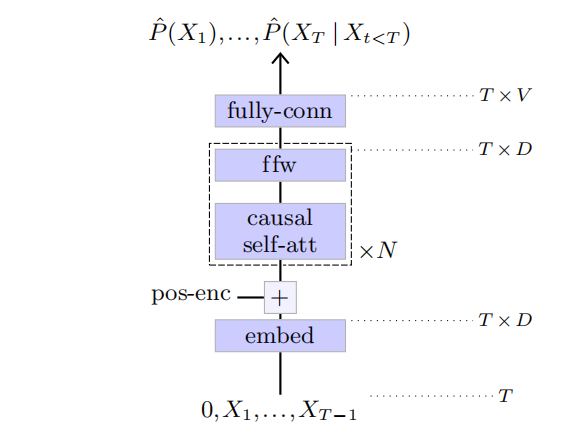
\includegraphics[width=0.9\textwidth]{fig/fig5.8.png}
    \caption[GPT 模型]{GPT 模型}
    \label{fig5.8}
\end{figure}

\subsubsection*{视觉 Transformer}

Transformer 已通过\keyterm{视觉 Transformer} (\keyterm{ViT}) 模型 \citep{arxiv-2010.11929} 用于图像分类(见图 \ref{fig5.9})。

它将三通道输入图像划分为 $M$ 个分辨率为 $P \times P$ 的图像块,然后将其展平,创建一系列形状为 $M \times 3P^2$ 的向量 $X_1,\dots,X_M$,该序列乘以形状为 $3P^2 \times D$ 的可训练矩阵 $W^E$,将其映射到 $M \times D$ 序列,该序列与一个可训练向量 $E_0$ 连接。然后通过多个自注意力模块处理生成的 $(M + 1) \times D$ 序列 $E_0,\dots,E_M$。详见 \ref{sec5.3} 节和图 \ref{fig5.6}。

结果序列中的第一个元素 $Z_0$ 对应于 $E_0$ 并且与图像的任何部分无关,最终由两隐藏层 MLP 处理以获得最终的 $C$ 个 logit 值。\cite{arxiv-1810.04805} 在 BERT 模型中引入了这样一个用于读取类别预测的 Token,称为 \keyterm{CLS token}。

\begin{figure}
    \centering
    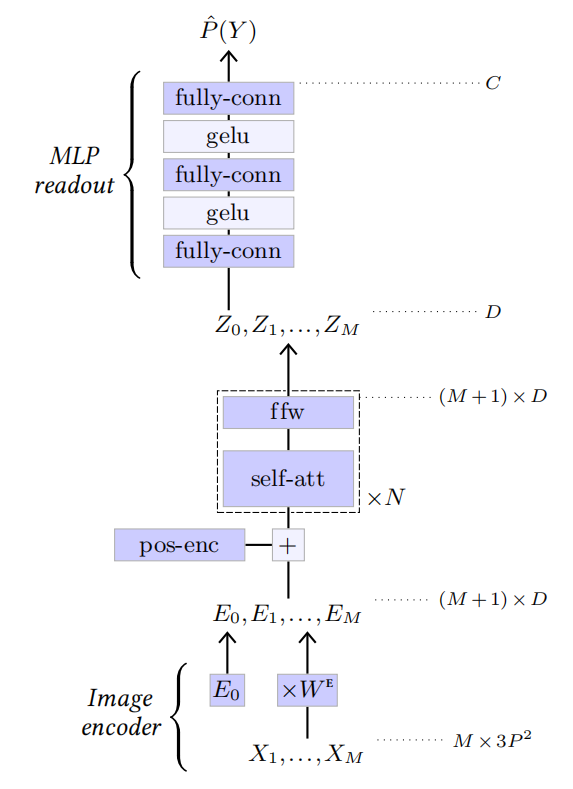
\includegraphics[width=0.9\textwidth]{fig/fig5.9.png}
    \caption[ViT 模型]{视觉 Transformer 模型 \citep{arxiv-2010.11929}}
    \label{fig5.9}
\end{figure}